\subsection{Klassenavn}

\begin{figure}[h]
\centering
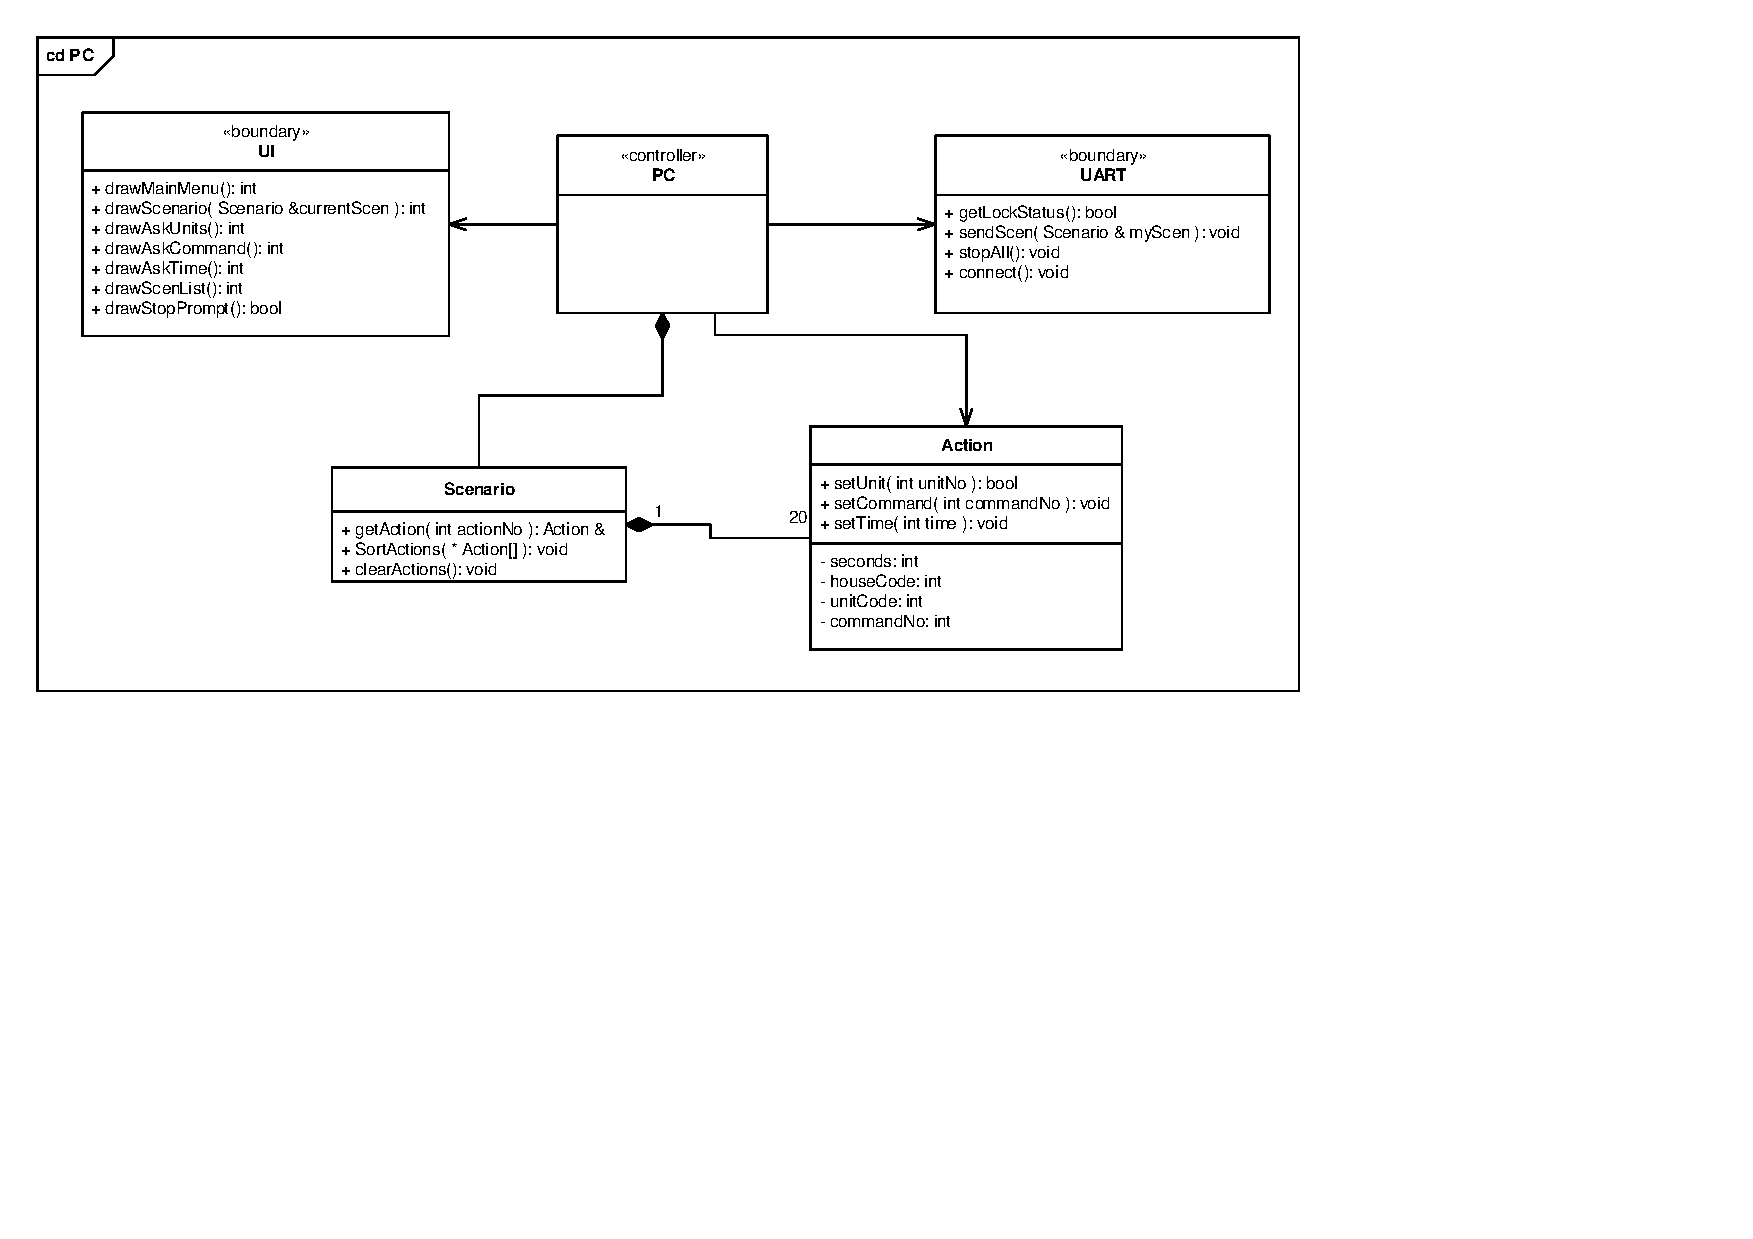
\includegraphics[scale=1,clip=true, trim=38 433 625 50]{../Systemarkitektur/diagrammer/PC_KlasseDiagram} %L B R T - HUSKE DET
\end{figure}

\begin{table}[h]
\begin{tabularx}{\textwidth}{p{0.6 cm} l X} %\hline
\multicolumn{3}{l}{\textbf{karstenNice}}\\
& Operation: & %Skriv tekst herunder
bool karstenNice( int theNumber ) 
\\ & Parametre: & %Skriv tekst herunder
Modtager et tal der skal sættes ind i Karsten 
\\ & Returværdi: & %Skriv tekst herunder
Returnerer hvorvidt det gik godt. 
\\ & Beskrivelse: & %Skriv tekst herunder
Something Something Something Something Something Something Something Something Something Something Something Something 
\\ \end{tabularx}
\end{table}

\begin{table}[h]
\centering
\begin{tabularx}{13 cm}{|l |X|} \hline
Attribut & Beskrivelse \\ \hline

myAtt & Denne attribut er bare for fed yo \\ \hline

\end{tabularx}
\end{table}